\subsection{Código de Hamming Estendido}

\begin{questions}
\question{
O Código de Hamming $(7,4,3)$ pode ser facilmente estendido
para o código $(8,4,4)$, bastando para tanto, acrescentar um
bit de paridade extra conforme a Figura \ref{fig:hamming84},
onde $x_4$, $x_5$, $x_6$ e $x_7$ são os bits de paridade,
sendo $x_7$ o bit extra acrescentado ao código estendido.

\begin{figure}
\centering
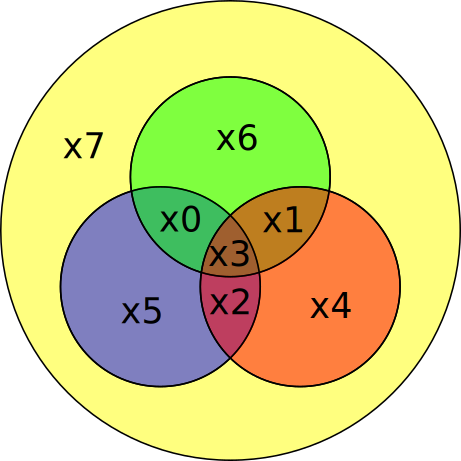
\includegraphics[width=0.33\textwidth]{../images/hamming84.pdf}
\caption{\label{fig:hamming84}Código de Hamming estendido $(8,4,4)$.}
\end{figure}

\begin{parts}
\part 
Apresente a matriz geradora para o código de Hamming estendido $(8,4,4)$.

\part 
Apresente a matriz de verificação de paridade para este código.

\part 
Qual é a distância mínima entre palavras no código de Hamming estendido $(8,4,4)$? Justifique.

\part 
Qual é o peso do código? Justifique.

\part
Faça um exemplo de codificação. Considere o seu número de matrícula, contendo $N$ algarismos, 
        na forma $a_{N-1} a_{N-2} \ldots a_1 a_0$. Considere como bits de dados: 
        $x_0 = a_{N-2} \mod 2$, $x_1 = a_{N-3} \mod 2$, $x_2 = a_{1} \mod 2$, $x_3 = a_{0} \mod 2$.
        Determine $x = x_{0}, x_{1}, \ldots, x_{7}$, a sequência de bits codificada.
        Suponha que $x$ será corrompido pelo ruído $z$, onde $z = z_0, z_1, \ldots, z_7$.
        Faça $z_i = 1$, $i = a_0 \mod 8$, e $a_0$ é o algarismo menos significativo
        do seu número de matrícula. A sequência corrompida pelo ruído será chamado de $y$.
        É possível determinar $x$ a partir de $y$? Em caso afirmativo, mostre como.

\part 
O que ocorrerá quando apenas um bit de $x$ for trocado? Será possível detectar erro?
        Será possível corrigir o erro? Justifique.

\part 
O que ocorrerá quando dois bits de $x$ forem trocados? Será possível detectar erro?
        Será possível corrigir os erros? Justifique.


\end{parts}
}

\begin{solution}
\begin{parts}
\part 
 Os primeiros 7 bits são iguais àqueles gerados pelo Código de Hamming $(7,4,3)$.
 O último bit será dado pela equação
         \begin{align}
        x_7 &= (x_0 + x_1 + x_2 + x_3 + x_4 + x_5 + x_6) \mod 2 \nonumber \\
            &= (3 x_0 + 3 x_1 + 3 x_2 + 4 x_3 ) \mod 2 \nonumber \\
            &= (x_0 + x_1 + x_2) \mod 2 .
        \end{align}
 
 Logo, a matriz geradora será
        \begin{equation}
        G = 
        \begin{pmatrix}
        1 & 0 & 0 & 0 \\
        0 & 1 & 0 & 0 \\
        0 & 0 & 1 & 0 \\
        0 & 0 & 0 & 1 \\
        0 & 1 & 1 & 1 \\
        1 & 0 & 1 & 1 \\
        1 & 1 & 0 & 1 \\ \hdashline[2pt/2pt]
        1 & 1 & 1 & 0
        \end{pmatrix}.
        \end{equation}


\part 
Para o código de Hamming estendido serão 4 equações de verificação de paridade.
Três delas são as mesmas dadas pelo Código de Hamming $(7,4,3)$.
A última equação deverá realizar a verificação de paridade de todos os bits
(ou alternativamente, $x_0, x_1, x_2, x_7$). 
Esta última equações para verificação de paridade será
\begin{equation}
x_0 + x_1 + x_2 + x_3 + x_4 + x_5 + x_6 + x_7 = 0 ,
\end{equation}
ou, alternativamente,
\begin{equation}
x_0 + x_1 + x_2 + x_7 = 0 .
\end{equation} 

A matriz de verificação de paridade será
        \begin{equation}
        H = 
        \left(
        \begin{array}{ccccccc;{2pt/2pt}c}
        0 & 1 & 1 & 1 & 1 & 0 & 0 & 0 \\
        1 & 0 & 1 & 1 & 0 & 1 & 0 & 0 \\
        1 & 1 & 0 & 1 & 0 & 0 & 1 & 0 \\ \hdashline[2pt/2pt]
        1 & 1 & 1 & 1 & 1 & 1 & 1 & 1
        \end{array}
        \right).
        \end{equation}
ou, alternativamente,
        \begin{equation}
        H = 
        \left(
        \begin{array}{ccccccc;{2pt/2pt}c}
        0 & 1 & 1 & 1 & 1 & 0 & 0 & 0 \\
        1 & 0 & 1 & 1 & 0 & 1 & 0 & 0 \\
        1 & 1 & 0 & 1 & 0 & 0 & 1 & 0 \\ \hdashline[2pt/2pt]
        1 & 1 & 1 & 0 & 0 & 0 & 0 & 1
        \end{array}
        \right).
        \end{equation}

\part 
A distância mínima do código de Hamming estendido $(8,4,4)$ é de 4.
Sendo duas palavras do código $v_1,v_2 \in C$, então $H(v_1 - v_2) = 0$,
pois o código é fechado em relação à soma e subtração.
Suponha que $v_1$ e $v_2$ se difiram apenas na posição $i$, então
$H(v_1 - v_2) = h_i$, onde $h_i$ é a $i$-ésima coluna de $H$. Como 
não existe coluna nula em $H$, temos um contradição. Logo, não é possível
que duas palavras do código $v_1$ e $v_2$ se difiram em apenas uma posição.
Vamos supor agora que elas se difiram em 2 posições, $i$ e $j$. Neste caso,
$H(v_1 - v_2) = h_i + h_j$, ou seja, a combinação das colunas $i$ e $j$ de $H$.
Entretanto, as colunas de $H$ são distintas, logo não é possível que a soma de
duas colunas seja nula. Mais uma vez, por contradição, verificamos que a distância
mínima entre duas palavras do código dado não pode ser 2.
Até aqui, seguimos os mesmos argumentos que aqueles dados para o código de Hamming $(7,4,3)$.
Vamos agora analisar o caso em que $v_1$ e $v_2$ se difiram em três posições $i$, $j$ e $k$.
Teremos agora $H(v_1 - v_2) = h_i + h_j + h_k$, e temos que $v_1,v_2 \in C$, então $H(v_1 - v_2) = 0$.
Note que o último elemento de cada coluna de $H$ é $1$, logo qualquer soma de 3 colunas
de $H$ terá em seu último elemento o valor $1$ e, por conseguinte, não poderemos ter o resultado
nulo. Por contradição, mais uma vez, concluímos que a distância mínima entre duas palavras 
no código de Hamming estendido $(8,4,4)$ não pode ser 3.
Para uma distância 4 é possível fazer uma combinação de 4 colunas de $H$ igualando a zero,
como por exemplo, as colunas 1, 2, 3 e 8, somadas resultarão em zero.

\part 
O peso do código é 4.

        \begin{enumerate}
        \item Não podemos ter peso 1 pois as palavras com peso 1 não estão no espaço nulo de
        $\mathbf{H}$. Suponha que a palavra $x$ seja não nula apenas na posição $i$. Então
        $\mathbf{H} x$ será igual à $i$-ésima coluna de $\mathbf{H}$. Mas não existe coluna
        nula em $\mathbf{H}$, desta forma não é possível ter $\mathbf{H} x = 0$ com palavras
        de peso 1.
        \item Suponha que o peso do código seja 2, com elementos não nulos nas posições $i$ e $j$.
        Neste caso, por ser uma palavra do código, devemos ter $\mathbf{H} x = 0$, assim a soma
        da $i$-ésima e $j$-ésima colunas de $\mathbf{H}$ deverá ser igual a zero.
        Como as colunas de $\mathbf{H}$ são todas diferentes, a soma de quaisquer duas colunas é
        não nula. Desta forma não é possível que o código tenha peso 2.
        \item Peso 3 também não é possível. Note que a última linha de $\mathbf{H}$ é toda igual a 1,
        logo ao somar 3 colunas de $\mathbf{H}$, no último índice estaremos somando 1 três vezes, e
        terá como resultado 1. Desta forma, será impossível obter como resultado o $0$ desejado.
        \item Peso 4 será possível.
        \end{enumerate}


\part 
Vamos supor aqui que o número de matrícula é 12345678. Neste caso, teremos
$x_0 = 0$, $x_1 = 1$, $x_2 = 0$ e $x_3 = 1$, podemos assim calcular os bits
de baridade e obter o vetor $x = [0 1 0 1 0 1 0 1]$.
Para o exemplo dado, teremos $z = [1 0 0 0 0 0 0 0]$, logo
$y = x + z = [1 1 0 1 0 1 0 1]$.
Para determinar $x$ a partir de $y$ devemos calcular a síndrome, $s = Hy = H(x+z) = Hz$.
\begin{equation}
s = Hy = \begin{pmatrix} 0 \\ 1 \\ 1 \\ 1 \end{pmatrix} .
\end{equation}
Como $s$ não é nula, sabemos que ocorreu erro.
$s$ é igual à primeira coluna de $H$, logo $z$ é um vetor todo nulo, exceto em sua
primeira posição, $z = [1 0 0 0 0 0 0 0]$. Após obter $z$, podemos achar $x$, dado que $y=x+z$.
Teremos então $x = [0 1 0 1 0 1 0 1]$. Quando o erro for ocasionado pela troca de apena um bit, 
poderemos corrigi-lo.

\part 
Quando apenas um bit for trocado, será possível detectar e corrigir o erro, conforme 
exemplificado no item anterior. Se o erro for em apenas um bit, a síndrome será uma 
das colunas de $H$. Bastará então identificar qual coluna para saber qual bit foi trocado.

\part 
Se dois bits forem trocados, será possível detectar o erro, pois a síndrome será
a combinação de duas colunas de $H$, que não será nula. Entretanto, não será possível
corrigir, pois para uma mesma síndrome existem diferentes combinações de duas colunas de $H$
que levam a um mesmo resultado. Por exemplo, se o erro trocar os dois primeiros bits,
$z = [1 1 0 0 0 0 0 0]$, teremos $y = x + z = [1 0 0 1 0 1 0 1]$. 
\begin{equation}
s = Hy = \begin{pmatrix} 1 \\ 1 \\ 0 \\ 0 \end{pmatrix} ,
\end{equation}
que pode ser obtido pela diferentes combinações de duas colunas de $H$:
$(1,2)$, $(3,8)$, $(4,7)$ e $(5,6)$.

\end{parts}
\end{solution}
\end{questions}
